\documentclass{article}
\usepackage{graphicx}
\graphicspath{images/} 
\usepackage[utf8]{inputenc}
\usepackage{aaai}
\usepackage{url}
\usepackage{array,booktabs,longtable,tabularx,tabulary}
\usepackage{multirow}
\begin{document}
\title{TITLE HERE PLEASE} 
\author{Hannah Gautreau}
\date{}
\maketitle

\section{Methods}
\subsection{Selection of Class Variable}
There were a number of candidate variables to use as a proxy for "success" in the first work term. The main candidates were when the student got a job, and their work term evaluation. 

Figure \ref{evals} shows the distribution of evaluations. The vast majority of the students have received evaluations of excellent or outstanding, and there was no correlation that emerged between the work term evaluation and any feature in the feature list. Due to the fact that the evaluations are close to random, and heavily biased toward excellent and outstanding, they were removed from consideration in the model.

Figure \ref{fig:timing} shows the distribution of when first work term students were matched with a job. This is a much more interesting class variable because there are significantly fewer students who were matched in the first round of the job search. In addition to this, there more correlation with getting a job in the first round and other features in the model. 

\begin{figure}[h]
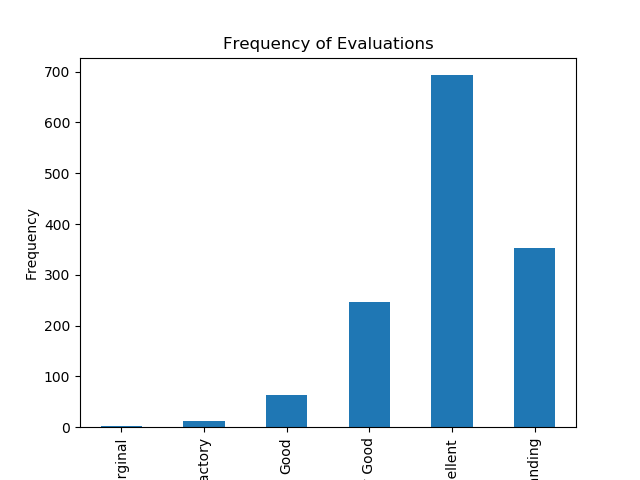
\includegraphics[width=9cm]{Evals.png}
\caption{Frequency of First Work Term Evaluations}\label{fig:evals}
\centering
\end{figure}

\begin{figure}[h]
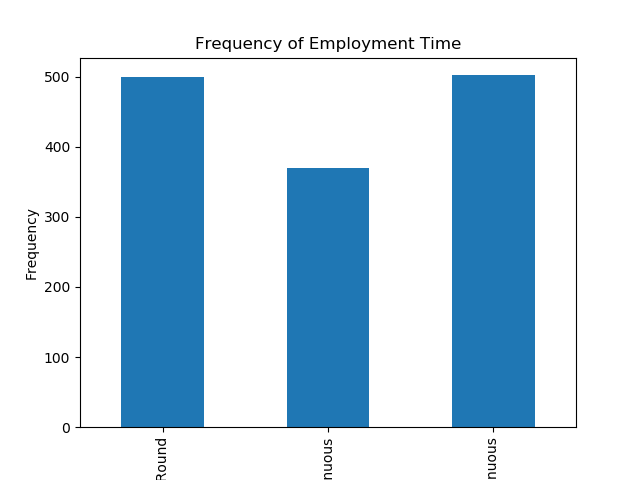
\includegraphics[width=9cm]{timing.png}
\caption{Frequency of First Work Term Employment Timing}\label{fig:timing}
\centering
\end{figure}


\subsection{Feature Selection}
The features with the best predictive value were selected using the Recursive Feature Elimination (RFE) Algorithm. This algorithm recursively removes features, builds a model using the remaining features, and calculates the accuracy of the model. The result of this is the combination of attributes that are the most useful to predicting the target variable \cite{hg:11}. All features were used in the algorithm. 

To determine which features should be used in the model, numerous iterations of the RFE algorithm were run to determine the optimal number of features. To determine the accuracy of the resulting model, a simple Logistic Regression was run with 5-fold cross validation. Figure \ref{fig:feature_selection} shows that the optimal number of features used is 9. Here is the ranked list of features chosen by the RFE Algorithm: 
\begin{enumerate}
	\item HS\_JOB
	\item PROGRAMMING
	\item EA\_COUNT
	\item COM\_EA
	\item DRA\_EA
	\item MUS\_EA
	\item OTH\_EA
	\item PRJ\_EA
	\item SOC\_EA
\end{enumerate}

\begin{figure}[h]
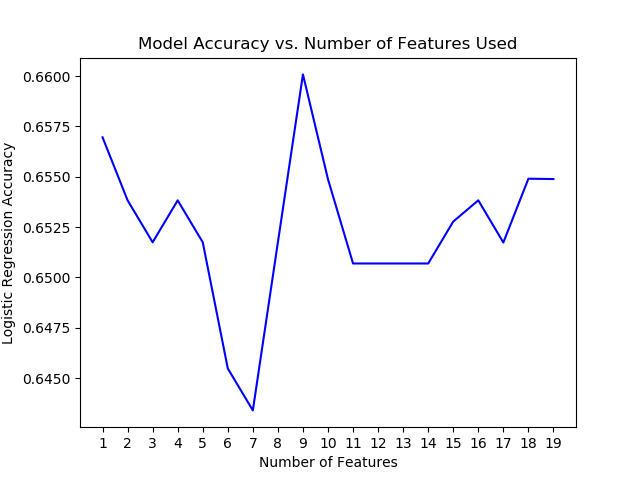
\includegraphics[width=9cm]{FeatureSelection.png}\label{fig:feature_selection}
\caption{Model Accuracy vs. Number of Features Used}
\centering
\end{figure}

\subsection{Algorithm Selection and Evaluation}

The following 6 classification algorithms were evaluated as candidates for the final model. 
\begin{enumerate}
	\item Logistic Regression (LR)
	\item Linear Discriminant Analysis (LDA)
	\item K Nearest Neighbours Classifier (KNN)
	\item Decision Tree Classifier (DT)
	\item Gaussian Naive Bayes (NB)
	\item Support Vector Machine (SVM)
\end{enumerate}

All algorithms were evaluated on their overall accuracy using 10-fold cross validation on the features listed in the previous section. 
\section{Results}
Table \ref{tab:algs}  shows the results of this analysis. 

\begin{table}[!htb]
\setlength\tabcolsep{0pt} % let LaTeX compute intercolumn whitespace
\footnotesize\centering
\smallskip 
\begin{tabular*}{\columnwidth}{@{\extracolsep{\fill}}rcccr}
\toprule
  Algorithm&Accuracy&Standard Deviation \\
\midrule
  LR  & 0.660534    &0.048550\\
  LDA & 0.666897 & 0.054624\\
  KNN & 0.604904 & 0.049695\\
  DTC & 0.579349 & 0.042431\\
  NB & 0.633086  & 0.056725\\
  SVM & 0.663244  & 0.045802\\
  \midrule
\bottomrule
\end{tabular*}
\caption{Algorithm Evaluation Results} \label{tab:algs}
\end{table}

Figure \ref{fig:algs} shows a box and whisker plot of the evaluation to give more insight into the results. This plot shows tat there is too much overlap in the LR, LDA, NB, and SVM algorithms to make a definitive decision about which algorithm produced the best model. 

\begin{figure}[h]
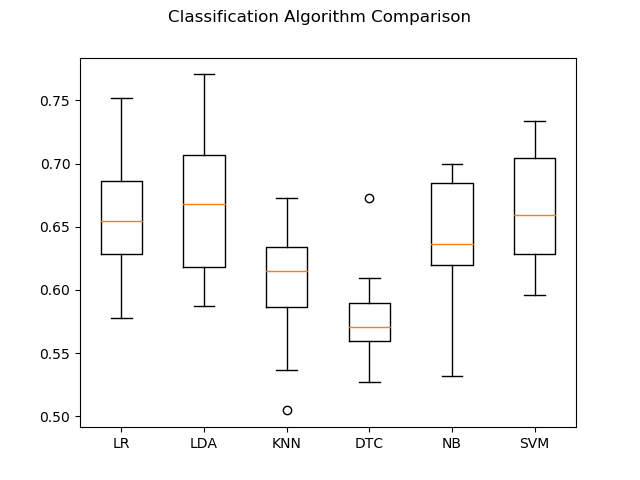
\includegraphics[width=9cm]{AlgorithmResults.png}
\caption{Algorithm Comparison Results}\label{fig:algs}
\centering
\end{figure}

The next four classifiers were evaluated using 20\% of the dataset
\subsection{Logistic Regression}

\begin{table}[!htb]
\setlength\tabcolsep{0pt} % let LaTeX compute intercolumn whitespace
\footnotesize\centering
\smallskip 
\begin{tabular*}{\columnwidth}{@{\extracolsep{\fill}}rcccr}
\toprule
  Class&Precision&Recall&F1-Score&Support \\
\midrule
  !FR  & 0.65&0.87&0.75&171\\
  FR & 0.53&0.24&0.33&104 \\
  \midrule
total&0.61&0.63&0.59&275\\
\bottomrule
\end{tabular*}
\caption{Logistic Regression Evaluation Metrics} \label{tab:lda}
\end{table}

\begin{figure}[h]
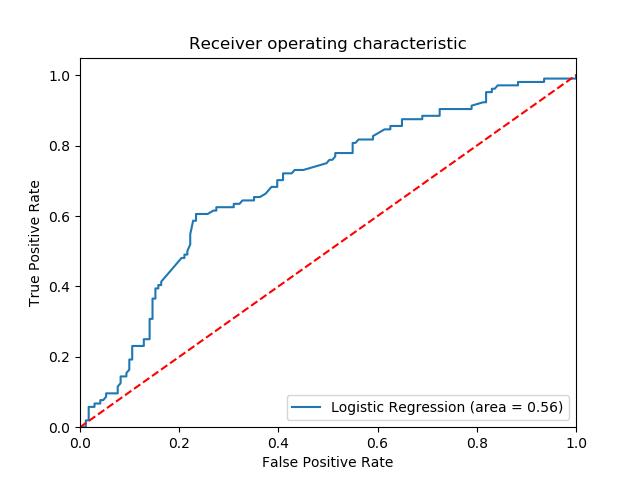
\includegraphics[width=9cm]{roc-lr.png}
\caption{ROC - Logistic Regression}\label{fig:lr}
\centering
\end{figure}

\subsection{Linear Discriminant Analysis}

\begin{table}[!htb]
\setlength\tabcolsep{0pt} % let LaTeX compute intercolumn whitespace
\footnotesize\centering
\smallskip 
\begin{tabular*}{\columnwidth}{@{\extracolsep{\fill}}rcccr}
\toprule
  Class&Precision&Recall&F1-Score&Support \\
\midrule
  !FR  & 0.66&0.86&0.75&171\\
  FR & 0.55&0.28&0.37&104 \\
  \midrule
total&0.62&0.64&0.60&275\\
\bottomrule
\end{tabular*}
\caption{Linear Discriminant Analysis Evaluation Metrics} \label{tab:lda}
\end{table}

\begin{figure}[h]
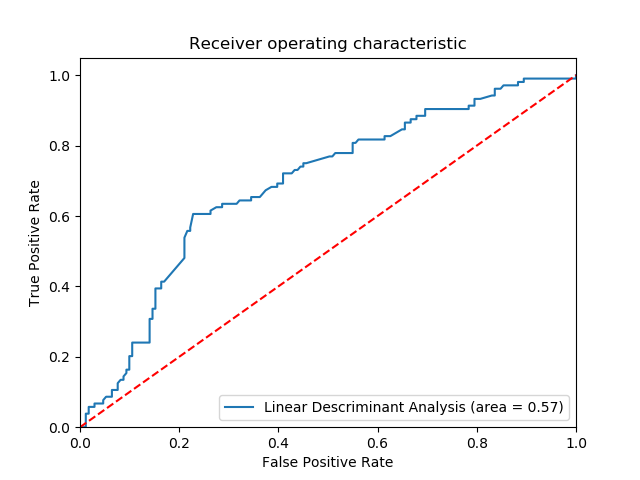
\includegraphics[width=9cm]{roc-lda.png}
\caption{ROC - Linear Discriminant Analysis}\label{fig:lda}
\centering
\end{figure}

\subsection{Naive Bayes}
\begin{table}[!htb]
\setlength\tabcolsep{0pt} % let LaTeX compute intercolumn whitespace
\footnotesize\centering
\smallskip 
\begin{tabular*}{\columnwidth}{@{\extracolsep{\fill}}rcccr}
\toprule
  Class&Precision&Recall&F1-Score&Support \\
\midrule
  !FR  & 0.69&0.80&0.74&171\\
  FR & 0.55&0.39&0.46&104 \\
  \midrule
total&0.63&0.65&0.63&275\\
\bottomrule
\end{tabular*}
\caption{Naive Bayes Evaluation Metrics} \label{tab:nb}
\end{table}

\begin{figure}[h]
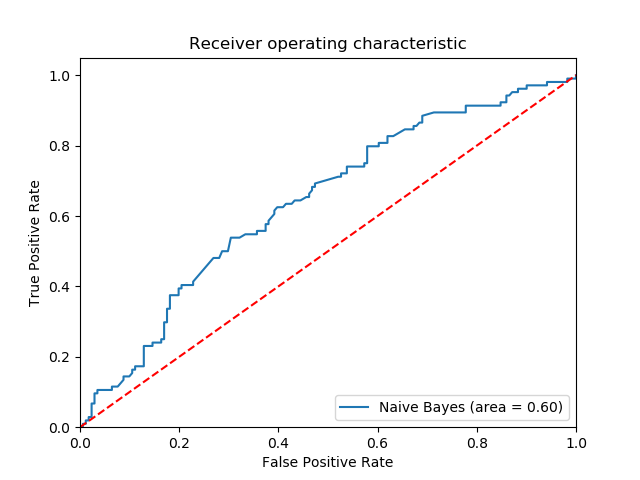
\includegraphics[width=9cm]{roc-nb.png}
\caption{ROC - Naive Bayes}\label{fig:nb}
\centering
\end{figure}
\subsection{Support Vector Machine}
\begin{table}[!htb]
\setlength\tabcolsep{0pt} % let LaTeX compute intercolumn whitespace
\footnotesize\centering
\smallskip 
\begin{tabular*}{\columnwidth}{@{\extracolsep{\fill}}rcccr}
\toprule
  Class&Precision&Recall&F1-Score&Support \\
\midrule
  !FR  & 0.65&0.90&0.76&171\\
  FR & 0.56&0.21&0.31&104 \\
  \midrule
total&0.62&0.64&0.59&275\\
\bottomrule
\end{tabular*}
\caption{Support Vector Machine Evaluation Metrics} \label{tab:svm}
\end{table}

\begin{figure}[h]
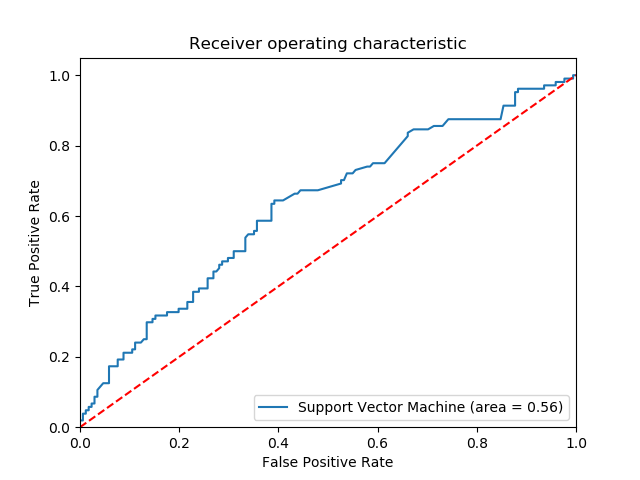
\includegraphics[width=9cm]{roc-svm.png}
\caption{ROC - Support Vector Machine}\label{fig:svm}
\centering
\end{figure}

\bibliography{CS686Bib}
\bibliographystyle{aaai}

\end{document}
